\documentclass{beamer}
%Imports and customization
\usepackage{tikz}
\usepackage{graphicx}
\usepackage{tikz-feynman}
\graphicspath{ 
    {./images/}
}

\beamertemplatenavigationsymbolsempty
\setbeamertemplate{sidebar right}{}
\setbeamertemplate{footline}{
    \hfill\usebeamertemplate***{navigation symbols}
    \hspace{1cm}\insertframenumber{}/\inserttotalframenumber
}
\setbeamertemplate{caption}{\raggedright\insertcaption\par}
\setbeamersize{text margin left=5mm,text margin right=5mm} 

\setbeamerfont{itemize/enumerate body}{size=\scriptsize}
\setbeamerfont{itemize/enumerate subbody}{size=\scriptsize}
\setbeamerfont{itemize/enumerate subsubbody}{size=\scriptsize}


%Custom Macros
\newcommand{\statwarn}{
    \tiny \color{red} Absolute numbers here mean NOTHING. Plots are based on small (100k events) samples, and are highly biased. All that matters is relative position!
}


\newcommand{\fullscreenimage}[2]{
    \frame{
        \frametitle{#1} 
        \begin{figure}
        \includegraphics[height=0.9\textheight,keepaspectratio]{#2}
        \end{figure}
    }
}


\newcommand{\displayone}[3]{
    \frame{
        \frametitle{#1} 
        \begin{columns}
            \begin{column}{0.5\textwidth}
                #2
            \end{column}
            \begin{column}{0.5\textwidth}
                \begin{figure}
                    \includegraphics[width=\linewidth,height=\textheight,keepaspectratio]{#3}
                \end{figure}
            \end{column}
        \end{columns}
    }
}

\newcommand{\displayonelarge}[3]{
    \frame{
        \frametitle{#1} 
        \begin{columns}
            \begin{column}{0.3\textwidth}
                #2
            \end{column}
            \begin{column}{0.7\textwidth}
                \begin{figure}
                    \includegraphics[width=\linewidth,height=\textheight,keepaspectratio]{#3}
                \end{figure}
            \end{column}
        \end{columns}
    }
}


\newcommand{\displaytwo}[4]{
    \frame{
        \frametitle{#1} 
        #2
        \begin{columns}
            \begin{column}{0.5\textwidth}
                \begin{figure}
                    \includegraphics[width=\linewidth,height=\textheight,keepaspectratio]{#3}
                \end{figure}
            \end{column}
            \begin{column}{0.5\textwidth}
                \begin{figure}
                    \includegraphics[width=\linewidth,height=\textheight,keepaspectratio]{#4}
                \end{figure}
            \end{column}
        \end{columns}
    }
}


\newcommand{\displaythree}[5]{
    \frame{
        \begin{columns}[T]
            \begin{column}{0.5\textwidth}
                \insertframetitle{#1}\\
                #2
            \end{column}
            \begin{column}{0.5\textwidth}
                \begin{figure}
                    \includegraphics[width=\linewidth,height=\textheight,keepaspectratio]{#3}
                \end{figure}
            \end{column}
        \end{columns}
        \begin{columns}[T]
            \begin{column}{0.5\textwidth}
                \begin{figure}
                    \includegraphics[width=\linewidth,height=\textheight,keepaspectratio]{#4}
                \end{figure}
            \end{column}
            \begin{column}{0.5\textwidth}
                \begin{figure}
                    \includegraphics[width=\linewidth,height=\textheight,keepaspectratio]{#5}
                \end{figure}
            \end{column}
        \end{columns}
    }
}


\newcommand{\announcesection}[1]{
    \section{#1}
    \frame{
        \begin{center}
            {\huge #1} 
        \end{center}
    }
}


%Begin Presentation
\begin{document}
    \title{Further Work on a New VBF Tagging Algorithm,\\ and Also Starting Work on Development of the B-Jet Trigger Online Monitoring Code}
    \author{Chris Milke}
    \date{2 March, 2020}

    \frame{\titlepage}
    \frame{\frametitle{Overview} \tableofcontents}

    \section{The Advantage and Challenge of Vector Boson Fusion}
\frame {
    \frametitle{Vector Boson Fusion (VBF)}

    \begin{columns}
        \begin{column}{0.4\textwidth}
            %{ \scriptsize VBF is the second highest Higgs production mechanism, but possesses a much better handle to identify the jets with than the leading mechanism, gluon-gluon fusion. }

            \begin{figure}
                \includegraphics[width=\linewidth,height=0.5\textheight,keepaspectratio]{higgs_production_modes.png}
                \caption{\scriptsize source - arXiv:1909.02845 [hep-ex] }
            \end{figure}
        \end{column}
        \begin{column}{0.6\textwidth}
            {\scriptsize
                VBF events can be identified based on the two hight-$p_T$, large $\Delta \eta$ jets (called  {\it signature jets})
            }
            \begin{center}\resizebox{0.40\textheight}{!}{ \begin{tikzpicture} \begin{feynman}
    \vertex (a);
    \vertex [right=of a] (b) {H};
    \vertex [above left=of a] (vb1);
    \vertex [below left=of a] (vb2);
    \vertex [left=of vb1] (q1i) {q};
    \vertex [left=of vb2] (q2i) {q};
    \vertex [above =of b] (q1f) {q};
    \vertex [below =of b] (q2f) {q};

    \diagram* {
        (q1i) -- (vb1) -- (q1f),
        (q2i) -- (vb2) -- (q2f), 
        (vb1) -- [boson] (a) -- [boson] (vb2),
        (a) -- [scalar] (b),
    };
\end{feynman} \end{tikzpicture}
 }\end{center}

            {\scriptsize
                At leading order, ggF results in only the decay products of the Higgs itself
            }
            \begin{center}\resizebox{0.40\textheight}{!}{ \begin{tikzpicture} \begin{feynman}
    \vertex (c);
    \vertex [above left=of c] (a);
    \vertex [below left=of c] (b);
    \vertex [left=of a] (gluon1) {g};
    \vertex [left=of b] (gluon2) {g};
    \vertex [right=of c] (higgs) {H};

    \diagram* {
        (gluon1) --[gluon] (a) 
        (gluon2) --[gluon] (b)
        (c) --[scalar] (higgs)
        (a) -- (b) -- (c) -- (a)
    };
\end{feynman} \end{tikzpicture}
 }\end{center}
        \end{column}
    \end{columns}
}

\frame {
    \frametitle{ My Goal: Increase Discrimination Between VBF and ggF }

    \begin{columns}
        \begin{column}{0.4\textwidth}
            ggF events can produce radiation than makes them look like vbf events.
            Events must be properly tagged to avoid polluting statistics.
        \end{column}
        \begin{column}{0.6\textwidth}
            \begin{center}\resizebox{0.40\textheight}{!}{ \begin{tikzpicture} \begin{feynman}
    \vertex (a);
    \vertex [right=of a] (b) {H};
    \vertex [above left=of a] (vb1);
    \vertex [below left=of a] (vb2);
    \vertex [left=of vb1] (q1i) {q};
    \vertex [left=of vb2] (q2i) {q};
    \vertex [above =of b] (q1f) {q};
    \vertex [below =of b] (q2f) {q};

    \diagram* {
        (q1i) -- (vb1) -- (q1f),
        (q2i) -- (vb2) -- (q2f), 
        (vb1) -- [boson] (a) -- [boson] (vb2),
        (a) -- [scalar] (b),
    };
\end{feynman} \end{tikzpicture}
 }\end{center}
            \begin{center}\resizebox{0.40\textheight}{!}{ 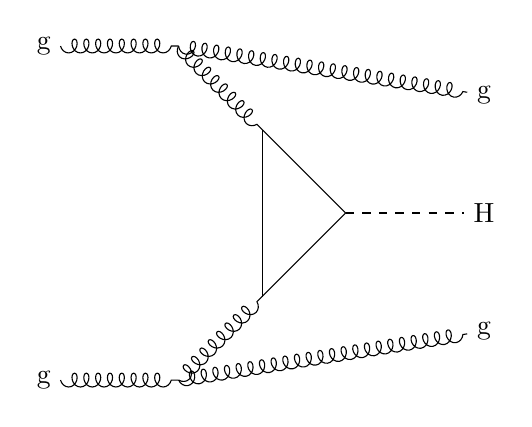
\begin{tikzpicture} \begin{feynman}
    \vertex (c);
    \vertex [above left=of c] (a);
    \vertex [below left=of c] (b);
    \vertex [above left=of a] (gluon1b);
    \vertex [below left=of b] (gluon2b);
    \vertex [left=of gluon1b] (gluon1) {g};
    \vertex [left=of gluon2b] (gluon2) {g};
    \vertex [right=of c] (higgs) {H};
    \vertex [above=of higgs] (rad1) {g};
    \vertex [below=of higgs] (rad2) {g};

    \diagram* {
        (gluon1) -- [gluon] (gluon1b) --[gluon] (a),
        (gluon2) -- [gluon] (gluon2b) --[gluon] (b),
        (c) --[scalar] (higgs),
        (gluon1b) -- [gluon] (rad1),
        (gluon2b) -- [gluon] (rad2),
        (a) -- (b) -- (c) -- (a)
    };
\end{feynman} \end{tikzpicture}
 }\end{center}
        \end{column}
    \end{columns}
}

    \frame {
    \frametitle{The Complication of Many Jets}
    \begin{columns}
        \begin{column}{0.5\textwidth}
            \underline{\large Initial State Radiation (ISR)} \\ \vspace{5mm}
            \resizebox{0.95\textwidth}{!}{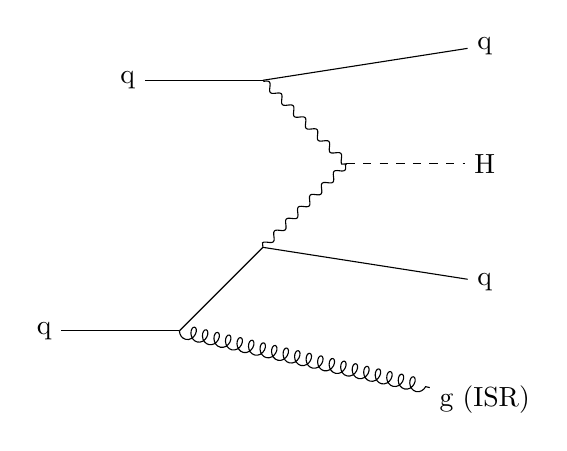
\begin{tikzpicture} \begin{feynman}
                \vertex (a);
                \vertex [right=of a] (b) {H};
                \vertex [above left=of a] (vb1);
                \vertex [below left=of a] (vb2);
                \vertex [left=of vb1] (q1i) {q};
                \vertex [below left=of vb2] (q2k);
                \vertex [left=of q2k] (q2i) {q};
                \vertex [above =of b] (q1f) {q};
                \vertex [below =of b] (q2f) {q};
                \vertex [below =of q2f] (g) {g (ISR)};

                \diagram* {
                    (q1i) -- (vb1) -- (q1f),
                    (q2i) -- (q2k) -- (vb2) -- (q2f),
                    (q2k) --[gluon] (g),
                    (vb1) -- [boson] (a) -- [boson] (vb2),
                    (a) -- [scalar] (b),
                };
            \end{feynman} \end{tikzpicture}}
        \end{column}
        \begin{column}{0.4\textwidth}
            \underline{\large Final State Radiation (FSR)} \\ \vspace{5mm}
            \resizebox{0.95\textwidth}{!}{\begin{tikzpicture} \begin{feynman}
                \vertex (a);
                \vertex [right=of a] (b) {H};
                \vertex [above left=of a] (vb1);
                \vertex [below left=of a] (vb2);
                \vertex [left=of vb1] (q1i) {q};
                \vertex [left=of vb2] (q2i) {q};
                \vertex [below right=of vb2] (q2k);
                \vertex [above =of b] (q1f) {q};
                \vertex [below =of b] (q2f) {q};
                \vertex [below =of q2f] (g) {g (FSR)};

                \diagram* {
                    (q1i) -- (vb1) -- (q1f),
                    (q2i) -- (vb2) -- (q2k) -- (q2f), 
                    (q2k) --[gluon] (g),
                    (vb1) -- [boson] (a) -- [boson] (vb2),
                    (a) -- [scalar] (b),
                };
            \end{feynman} \end{tikzpicture}}
        \end{column}
    \end{columns}
}

    \announcesection{Centrality}
\displayonelarge{What is Centrality?}
{
    { \scriptsize
        In VBF events, we expect that radiation (ISR or FSR) should be closely centered around the signature jets, compared to background events where the radiation is random.
    }
}{remote/figures/colinearity_pt_aviv_mjj_0}

\displaytwo{Centrality Depends Heavily on Primary Jets}
{
    For example, choosing the jet pair with the largest $M_{jj}$ compresses the centrality distribution between -1 and 1.
    
}
{remote/figures/colinearity_pt_aviv_mjj_0}
{remote/figures/colinearity_mjj_aviv_mjj_0}

\frame{
    \frametitle{Centrality in Use}
    \begin{figure}
    \includegraphics[height=0.8\textheight,keepaspectratio]
        {remote/performance/roc_cmilke_tag}
    \caption{ Centrality limit courtesty of ATL-COM-PHYS-2019-1252 }
    \end{figure}
}

% yes a roc curve

    \section{Online Monitoring Migration}

\displaythree{B-Jet Trigger Online Monitoring}
{ \small The Athena monitoring code is used to monitor the functionality of the ATLAS and the HLT while running }
{old_variables/jet_pt} 
{old_variables/jf_ntrkv} 
{old_variables/tag_MV2c10} 

\frame{
    \frametitle{ Original B-Jet Trigger Online Monitered Variables }
    \begin{center} \resizebox{0.95\textheight}{!}{
        \begin{tabular}{ |l|l|l| }
        \hline
      \textbf {Algorithm} & \textbf {Histograms} & \textbf {Title} \\
        \hline
                         &   sv1\_mass     &  BtagFex SV Mass \\
                         &   sv1\_evtx     &  BtagFex SV Energy Fraction \\
                         &   sv1\_nvtx     &  BtagFex SV Two-Track Vertex Number \\
                         &   tag\_IP2D     &  BtagFex IP2D Likelihood Ratio \\
                         &   tag\_IP3D     &  BtagFex IP3D Likelihood Ratio \\
                         &   tag\_SV1      &  BtagFex SV1 Likelihood Ratio \\
                         &   tag\_IP3DSV1  &  BtagFex IP3D+SV1 Discriminant \\
                         &   tag\_MV2c10   &  BtagFex MV2c10 Discriminant \\
                         &   tag\_MV2c20   &  BtagFex MV2c20 Discriminant \\
  EFBtagFexSplit\_EFID,  &   jet\_pt       &  BtagFex Jet PT \\
  EFBtagFex\_EFID        &   jet\_eta      &  BtagFex Jet Eta \\
                         &   tag\_IP2\_c   &  BtagFex IP2D Likelihood Ratio between b and c-jets \\
                         &   tag\_IP2\_cu  &  BtagFex IP2D Likelihood Ratio between c and light-jets \\
                         &   tag\_IP3\_c   &  BtagFex IP2D Likelihood Ratio between b and c-jets \\
                         &   tag\_IP3\_cu  &  BtagFex IP2D Likelihood Ratio between c and light-jets \\
                         &   sv1\_ntkv     &  BtagFex SV Number of tracks used in the SV \\
                         &   sv1\_Lxy      &  BtagFex SV Transverse distance between PV and SV \\
                         &   sv1\_L3d      &  BtagFex SV Distance between PV and SV \\
                         &   sv1\_sig3     &  BtagFex SV 3D Vertex Significance \\
                         &   sv1\_dR       &  BtagFex SV delta R \\
                         &   jf\_n2tv      &  BtagFex JetFitter Number of 2-track vertex \\
                         &   jf\_ntrkv     &  BtagFex JetFitter Number of tracks from displaced vertices \\
                         &   jf\_nvtx      &  BtagFex JetFitter Number of displaced vertices \\
                         &   jf\_nvtx1t    &  BtagFex JetFitter Number of displaced vertices wih 1-track \\
                         &   jf\_mas       &  BtagFex JetFitter Jet mass \\
                         &   jf\_efrc      &  BtagFex JetFitter Jet efrac \\
                         &   jf\_dR        &  BtagFex JetFitter Delta R \\
                         &   jf\_sig3      &  BtagFex JetFitter 3D vertex significance \\
             \hline
                         &   gsc\_ntrk     &  GSCFex Number of tracks \\
                         &   gsc\_width    &  GSCFex Track width \\
     TrigGSCFex          &   gsc\_ptsm     &  GSCFex Sum of tranverse momentum of tracks \\
                         &   gsc\_ptdiff   &  GSCFex PT difference between uncal jet and cal jets \\
                         &   gsc\_ptratio  &  GSCFex PT ratio \\
            \hline
    \end{tabular}
    } \end{center}
}

\frame{
    \frametitle{Current Set of Variables (Validated!)}
    (Fullsize images in backup...)
    \begin{columns}
        \begin{column}{0.6\textwidth}
            \resizebox{0.8\textheight}{!}{
                \begin{tabular}{ |l|l| }
                    \hline
                    \textbf {Histograms} & \textbf {Title} \\
                    \hline
                    jet\_count    &    BtagFexMT Number of Jets \\
                    track\_count  &    BtagFexMT Number of Tracks \\
                    vertex\_count &    BtagFexMT Number of Vertices \\
                    jet\_pt       &  BtagFexMT Jet PT \\
                    jet\_eta      &  BtagFexMT Jet Eta \\
                    track\_Et     &    BtagFexMT Track Transverse Energy \\
                    track\_eta    &    BtagFexMT Track Eta \\
                    track\_phi    &    BtagFexMT Track Phi \\
                    track\_d0     &    BtagFexMT Track D0 \\
                    track\_d0err  &    BtagFexMT Track D0 Error \\
                    track\_d0sig  &    BtagFexMT Track D0 Significance \\
                    track\_z0     &    BtagFexMT Track Z0 \\
                    track\_z0err  &    BtagFexMT Track Z0 Error \\
                    track\_z0sig  &    BtagFexMT Track Z0 Significance \\
                    \hline
                \end{tabular}
            }
        \end{column}
        \begin{column}{0.4\textwidth}
            \begin{figure}
                \includegraphics[height=0.8\textheight,keepaspectratio]{variables_signed_off}
            \end{figure}
        \end{column}
    \end{columns}
}


\displayonelarge{Latest Merge Request was Successful}
{ \small Most recent merge added no functionality,
    but moved monitoring code to a more appropriate algorithm 
    {\tiny (TrigBjetBtagHypoAlgMT)}.\\ \vspace{7mm}
    More variables and adjusted axes in next merge.  }
{merge_request}


    \section{Conclusion}
    \frame{
        \frametitle{Conclusions}
        \begin{itemize} {
            \item VBF events are a rich production mechanism for Higgs, which can be utilized more fully
            \item Three-jet VBF events are largely unexplored by current analyses, but can noticeably increase available statistics
            \item These events have a complex topology which presents many interesting handles for signal/background discrimination (e.g. Centrality, which has already been shown to improve performance)
            \item I have just started migrating the B-Jet Trigger Online Monitoring code to AthenaMT, and am getting a jump-start to this process at the AthenaMT workshop at CERN
        } \end{itemize}
    }

    \announcesection{Backup}
    \frame {
    \frametitle{How is VBF Currently Handled?}
    \begin{columns}
        \begin{column}{0.7\textwidth}
            VBF$\rightarrow$H$\rightarrow$invisible

            {\tiny
            (source - Phys. Lett. B 793 (2019) 499)
            \begin{quote}
                 - a leading jet with $p_T$ > 80 GeV, \\
                 - a subleading jet with $p_T$ > 50 GeV, \\
                 - no additional jets with $p_T$ > 25 GeV, \\
            \end{quote}
            }
        \end{column}
        \begin{column}{0.3\textwidth}
            \resizebox{0.7\textwidth}{!}{\begin{tikzpicture} \begin{feynman}
                \vertex (a);
                \vertex [right=of a] (b) {H};
                \vertex [above right=of b] (inv1) {$\chi$};
                \vertex [below right=of b] (inv2) {$\bar \chi$};
                \vertex [above left=of a] (vb1);
                \vertex [below left=of a] (vb2);
                \vertex [left=of vb1] (q1i) {q};
                \vertex [left=of vb2] (q2i) {q};
                \vertex [above=of inv1] (q1f) {q};
                \vertex [below=of inv2] (q2f) {q};

                \diagram* {
                    (q1i) -- (vb1) -- (q1f),
                    (q2i) -- (vb2) -- (q2f), 
                    (vb1) -- [boson] (a) -- [boson] (vb2),
                    (a) -- [scalar] (b) --[boson] { (inv1), (inv2)}
                };
            \end{feynman} \end{tikzpicture}}
        \end{column}
    \end{columns}
    \vspace{\fill}
    \begin{columns}
        \begin{column}{0.7\textwidth}
            VBF$\rightarrow$H$\rightarrow$diphoton

            {\tiny
            (source - DOI: 10.1103/PhysRevD.98.052005)
            \begin{quote}
                Events are required to contain at least two hadronic jets,
                and the selections applied are based on the two leading jets $(j_1, j_2)$ in the event.
            \end{quote}
            }
        \end{column}
        \begin{column}{0.3\textwidth}
            \resizebox{0.7\textwidth}{!}{\begin{tikzpicture} \begin{feynman}
                \vertex (a);
                \vertex [right=of a] (b) {H};
                \vertex [above right=of b] (gam1) {$\gamma$};
                \vertex [below right=of b] (gam2) {$\gamma$};
                \vertex [above left=of a] (vb1);
                \vertex [below left=of a] (vb2);
                \vertex [left=of vb1] (q1i) {q};
                \vertex [left=of vb2] (q2i) {q};
                \vertex [above=of gam1] (q1f) {q};
                \vertex [below=of gam2] (q2f) {q};

                \diagram* {
                    (q1i) -- (vb1) -- (q1f),
                    (q2i) -- (vb2) -- (q2f), 
                    (vb1) -- [boson] (a) -- [boson] (vb2),
                    (a) -- [scalar] (b) --[boson] { (gam1), (gam2)}
                };
            \end{feynman} \end{tikzpicture}}
        \end{column}
    \end{columns}
    \vspace{\fill}
    \begin{columns}
        \begin{column}{0.7\textwidth}
            VBF$\rightarrow$H$\rightarrow b \bar b$

            {\tiny
            (source - DOI: 10.1103/PhysRevD.98.052003)
            \begin{quote}
                The two highest-$p_T$ b-tagged jets form the Higgs boson candidate.
                Among the remaining jets, the pair of non-b-tagged jets with highest
                invariant mass is taken as the VBF jet pair.
            \end{quote}
            }
        \end{column}
        \begin{column}{0.3\textwidth}
            \resizebox{0.7\textwidth}{!}{\begin{tikzpicture} \begin{feynman}
                \vertex (a);
                \vertex [right=of a] (b) {H};
                \vertex [above right=of b] (b1) {$b$};
                \vertex [below right=of b] (b2) {$\bar b$};
                \vertex [above left=of a] (vb1);
                \vertex [below left=of a] (vb2);
                \vertex [left=of vb1] (q1i) {q};
                \vertex [left=of vb2] (q2i) {q};
                \vertex [above=of b1] (q1f) {q};
                \vertex [below=of b2] (q2f) {q};

                \diagram* {
                    (q1i) -- (vb1) -- (q1f),
                    (q2i) -- (vb2) -- (q2f), 
                    (vb1) -- [boson] (a) -- [boson] (vb2),
                    (a) -- [scalar] (b),
                    (b2) --[fermion] (b) --[fermion] (b1)
                };
            \end{feynman} \end{tikzpicture}}
        \end{column}
    \end{columns}
}

    %Slides like peilong’s slide 3 and 4 (about event generation and selection mechanisms

%Show eta distributions, then show that gamma plot that shows the gap in photon coverage from tight/loose photon (as explanation for why I filter on truth photons)





%\displaythree{Comparison of $d_0$}
%    { \begin{itemize}
%        \item Used for IP2D
%        \item Significance is what is ultimately used in tagging
%        \item Significance = $d_0$ / error
%        \item $d_0$ Error for FTK-IDTrig appears "shifted"
%    \end{itemize} }
%    {track_study/plot_d0_0}
%    {track_study/plot_d0_err_0}
%    {track_study/plot_d0_sig_0}
%\displaythree{Comparison of $z_0\sin\theta$}
%    { \begin{itemize}
%        \item Used for IP3D
%        \item Base value looks similar again
%        \item Shape of the errors distribution even more distinctive from HLT
%    \end{itemize} }
%    {track_study/plot_z0sintheta_0}
%    {track_study/plot_z0sintheta_err_0}
%    {track_study/plot_z0sintheta_sig_0}

\end{document}
